{
\begin{figure}[t!]
%\begin{minipage}{0.54\textwidth}
\begin{center}
\centerline{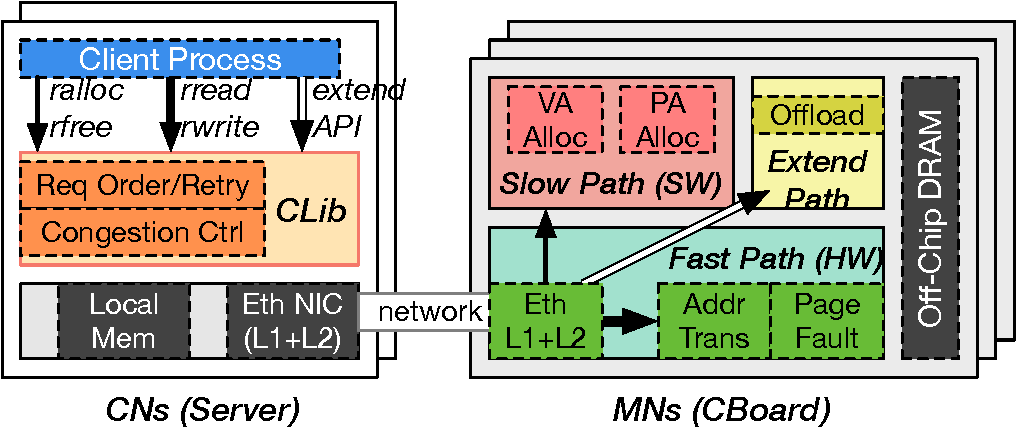
\includegraphics[width=1.0\columnwidth]{Figures/OverallArch.pdf}}
%\vspace{-0.1in}
\mycaption{fig-arch}{\sys\ Architecture.}
{
}
\end{center}
%\vspace{-0.05in}
\end{figure}
}


\section{\sys\ Overview}
\label{sec:clio:hdm}

\sys\ co-designs software with hardware, \CN{}s with \MN{}s, and network stack with virtual memory system, 
so that at the \MN{}, the entire data path is handled in hardware with high throughput, low (tail) latency, and minimal hardware resources. 
This section gives an overview of \sys's interface and architecture (Figure~\ref{fig-clio-arch}).

\subsection{\sys\ Interface}
\label{sec:clio:abstraction}


Similar to recent \md\ proposals~\cite{AIFM,sebastian-hotcloud20}, our current implementation adopts a non-transparent interface where
applications (running at \CN{}s) allocate and access disaggregated memory via explicit API calls. Doing so gives users opportunities to perform application-specific performance optimizations. 
By design, \sys’s APIs can also be called by a runtime like the AIFM runtime~\cite{AIFM} or by the kernel/hardware at \CN\ like LegoOS' pComponent~\cite{Shan18-OSDI} to support a transparent interface and allow the use of unmodified user applications.
We leave such extension to future work.

Apart from the regular (local) virtual memory address space, each process has a separate {\em \textbf{R}emote virtual memory \textbf{A}ddress \textbf{S}pace} ({\em \rspace} for short).
Each application process has a unique global {\em PID} across all \CN{}s which is assigned by \sys\ when the application starts.
Overall, programming in \rspace\ is similar to traditional multi-threaded programming except that memory read and write are explicit and that processes running on different \CN{}s can share memory in the same \rspace.
Figure~\ref{fig-clio-code-eg} illustrates the usage of \sys\ with a simple example.


An application process can perform a set of virtual memory operations in its \rspace,
including \alloc, \sysfree, \Cliosysread, \Cliosyswrite, 
and a set of atomic and synchronization primitives (\eg, \syslock, \sysunlock, \fence).
\alloc\ works like \texttt{malloc} and returns a VA in \rspace. \Cliosysread\ and \Cliosyswrite\ can then be issued to any allocated VAs.
As with the traditional virtual memory interface, allocation and access in \rspace\ are in byte granularity.
We offer {\em synchronous} and {\em asynchronous} options for \alloc, \sysfree, \Cliosysread, and \Cliosyswrite.
%, with which users can choose between performance and consistency levels.
%A synchronous API blocks until the result is ready.
%An asynchronous API is non-blocking, and the application calls \poll\ to get its result.

{
\begin{figure}[t]
\begin{center}
\footnotesize
\lstinputlisting[
numbers=left,
xleftmargin=6.0ex,
xrightmargin=0.1in,
frame=none,
framexleftmargin=15pt
]{code-eg.cpp}
%\vspace{-0.1in}
\mycaption{fig-code-eg}{Example of Using \sys.}
{
}
\end{center}
%\vspace{-0.1in}
\end{figure}
}

\ulinebfpara{Intra-thread request ordering.}
Within a thread, synchronous APIs follow strict ordering.
An application thread that calls a synchronous API blocks until it gets the result.
Asynchronous APIs are non-blocking. A calling thread proceeds after calling an asynchronous API and later calls \poll\ to get the result. 
Asynchronous APIs follow a release order.
%By default, all the APIs execute in an asynchronous fashion (\ie, there can be multiple outstanding operations),
%and we follow a release ordering of memory operations within each thread.
Specifically, asynchronous APIs may be executed out of order as long as
1) all asynchronous operations before a \release\ complete before the \release\ returns,
and 2) \release\ operations are strictly ordered.
On top of this release order, 
we guarantee that there is no concurrent asynchronous operations with dependencies (Write-After-Read, Read-After-Write, Write-After-Write) and target the same page.
The resulting memory consistency level is the same as architecture like ARMv8~\cite{ARMv8}.
In addition, we also ensure consistency between metadata and data operations, by ensuring that potentially conflicting operations execute synchronously in the program order. For example, if there is an ongoing \sysfree\ request to a VA, no read or write to it can start until the \sysfree\ finishes.
Finally, failed or unresponsive requests are transparently retried, and they follow the same ordering guarantees.

\ulinebfpara{Thread synchronization and data coherence.}
Threads and processes can share data even when they are not on the same \CN.
Similar to traditional concurrent programming, \sys\ threads can use synchronization primitives to build critical sections (\eg, with \syslock) 
and other semantics (\eg, flushing all requests with \fence).

An application can choose to cache data read from \Cliosysread\ at the \CN\ (\eg, by maintaining \texttt{local\_rbuf} in the code example).
Different processes sharing data in a \rspace\ can have their own cached copies at different \CN{}s.
Similar to ~\cite{Shan18-OSDI}, \sys\ does not make these cached copies coherent automatically and lets applications choose their own coherence
protocols.
We made this deliberate decision because automatic cache coherence on every read/write would incur  high performance overhead with commodity Ethernet infrastructure
and application semantics could reduce this overhead.

\subsection{\sys\ Architecture}

In \sys\ (Figure~\ref{fig-clio-arch}), \CN{}s are regular servers each equipped with a regular Ethernet NIC and connected to a top-of-rack (ToR) switch.
\MN{}s are our customized devices directly connected to a ToR switch.
%
Applications run at \CN{}s on top of our user-space library called {\em \syslib}.
It is in charge of request ordering, request retry, congestion, and incast control. 

By design, an \MN\ in \sys\ is a \sysboard\ consisting of an ASIC which runs the hardware logic for all data accesses (we call it the {\em fast path} and prototyped it with FPGA),
an ARM processor which runs software for handling metadata and control operations (\ie, the {\em slow path}),
and an FPGA which hosts application computation offloading (\ie, the {\em extend path}).
An incoming request arrives at the ASIC and travels through standard Ethernet physical and MAC layers 
and a Match-and-Action-Table (MAT) that decides which of the three paths the request should go to based on the request type.
If the request is a data access (fast path), it stays in the ASIC and goes through a hardware-based virtual memory system
that performs three tasks in the same pipeline: address translation, permission checking, and page fault handling (if any).
Afterward, the actual memory access is performed through the memory controller, and the response is formed and sent out through the network stack.
Metadata operations such as memory allocation are sent to the slow path. % and handled in software that runs on Linux at the ARM processor.
Finally, customized requests with %customized, high-level operations such as pointer chasing and 
offloaded computation are handled in the extend path.